\documentclass{article}
\usepackage{hyperref}
\usepackage{algorithm}
\usepackage{graphicx}
 %\usepackage{algorithmic}
 \usepackage{algpseudocode}
\begin{document}
\title{Simple Shell Documentation}
\author{Li Shitao}
\maketitle
\section{Description}
This program is a simplified shell command interpreter which is developed and tested on Ubuntu 14.04. The source codes of the program is avaliable on \url{https://github.com/list12356/simpleshell.git}
\section{Main Function}
The main function of this program is shown as following:
\begin{itemize}
\item resolve the internal command
\item resolve the external command
\item support the , including both $>$ and $>>$
\item support the command line pipe
\end{itemize}
\section{User Guide}
\subsection{Input the command}
This program include two exucetable files, the write and read. Before using the program, please make sure that you have a named pipe(FIFO file) avaliable and can open the write program and read program in two different terminal respectively. First, you should type the name of the FIFO file in both program and make sure that it is valid. And then you can type the commands in the write program so that the result will show on the read program. A simple example is showed in Figure \ref{fig:a}
\begin{figure}[htbp]
\label{fig:a}
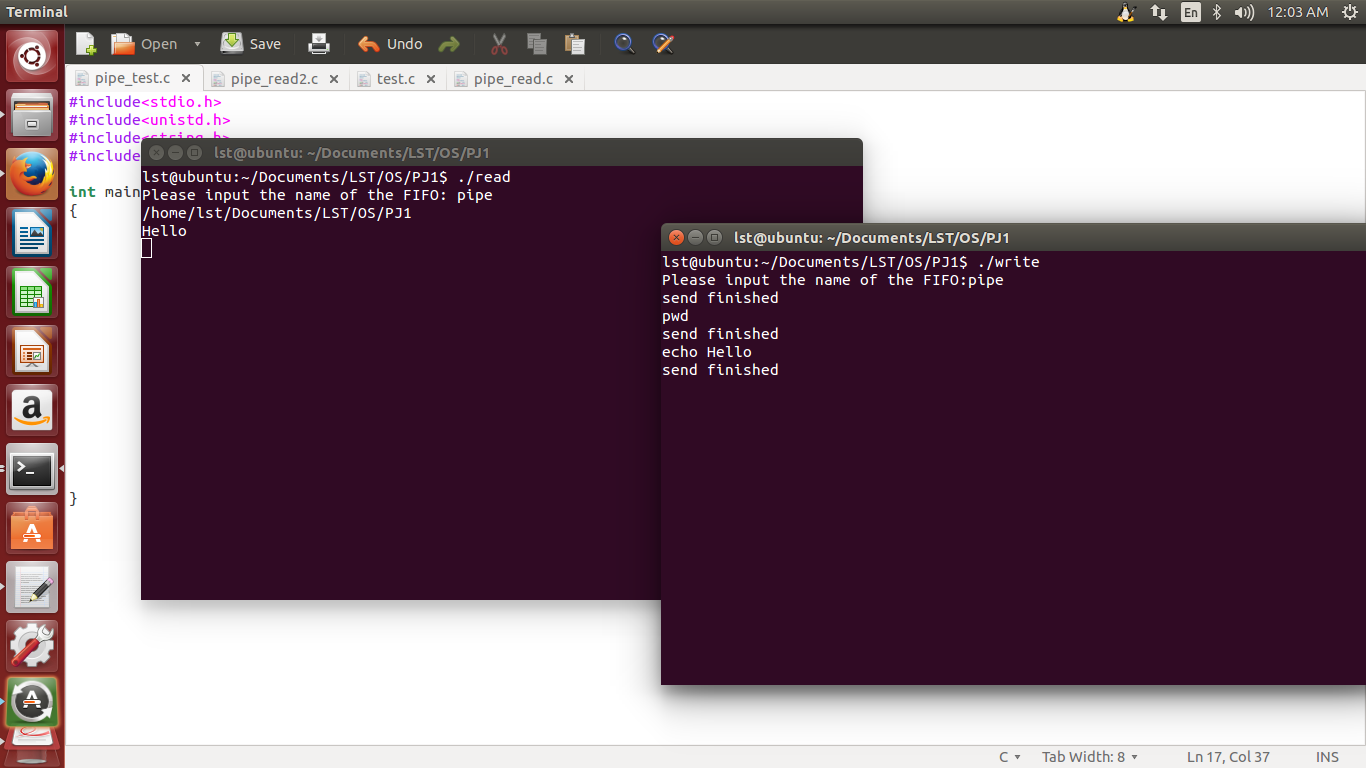
\includegraphics[width =400pt ,keepaspectratio ]{1.png}
\caption{Simple Example}
\end{figure}
\subsection{Output redirection}
The program can resolve two redirection symbols, $>$ and $>>$. For the symbol $>$, the program will first detect whether there already exists a file which match the name after the symbol. If there already exists a such file, the program will first delete it and create a new one to output the result. If there is no such file, the program wil create a new one. For the symbol $>>$, the program will output the result on the tail of the file, if it exists, or create a new one. An example is shown as below. We first use three ``pwd $>>$ tmp.txt'' command, and use ``cat tmp.txt'' we can see from Figure \ref{fig:b}that the results are added on the tail of the file ``tmp.txt''. And we use the ``ls $>$ tmp.txt'', and repeat the progress , we can see from Figure \ref{fig:c}that the tmp.txt file is rewritten by the program.
\begin{figure}[htbp]
\label{fig:b}
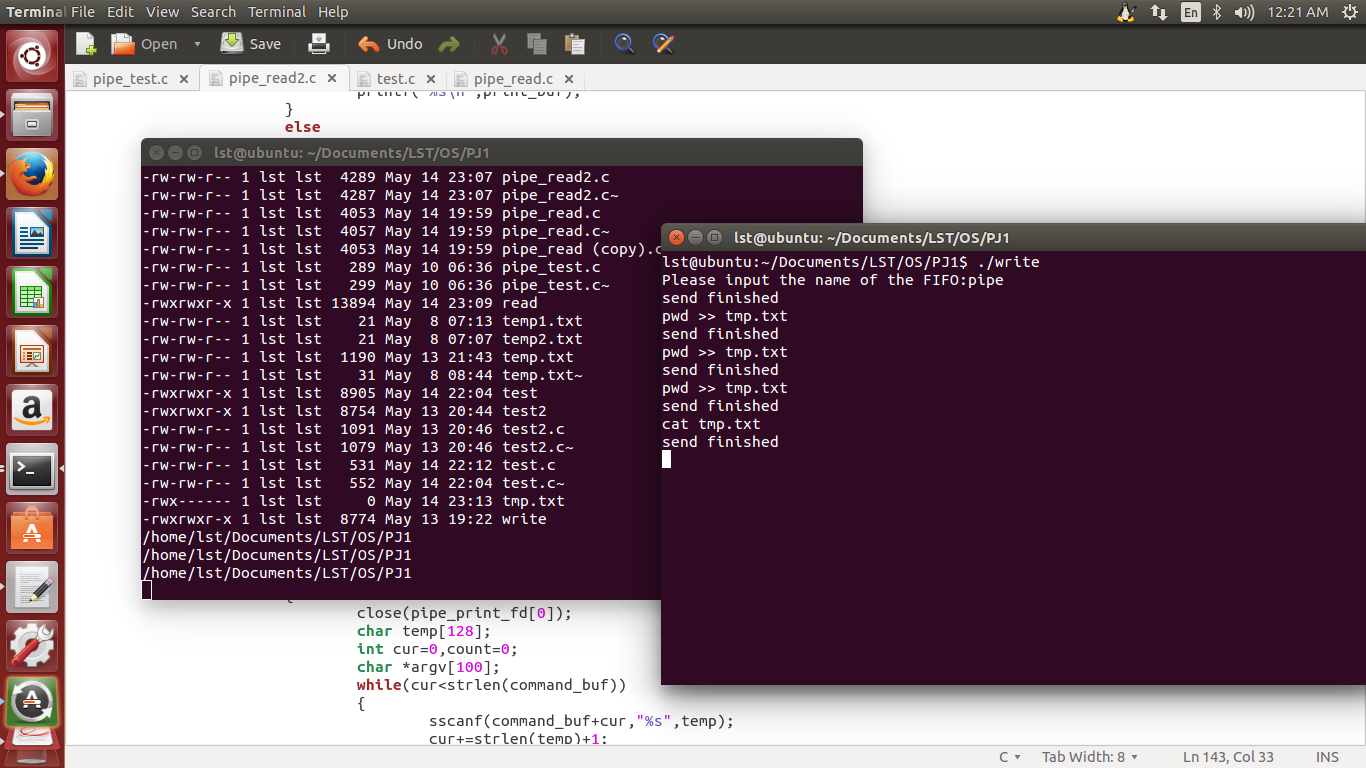
\includegraphics[width =400pt ,keepaspectratio ]{2.png}
\caption{Output Redirection}
\end{figure}
\\
\begin{figure}[htbp]
\label{fig:c}
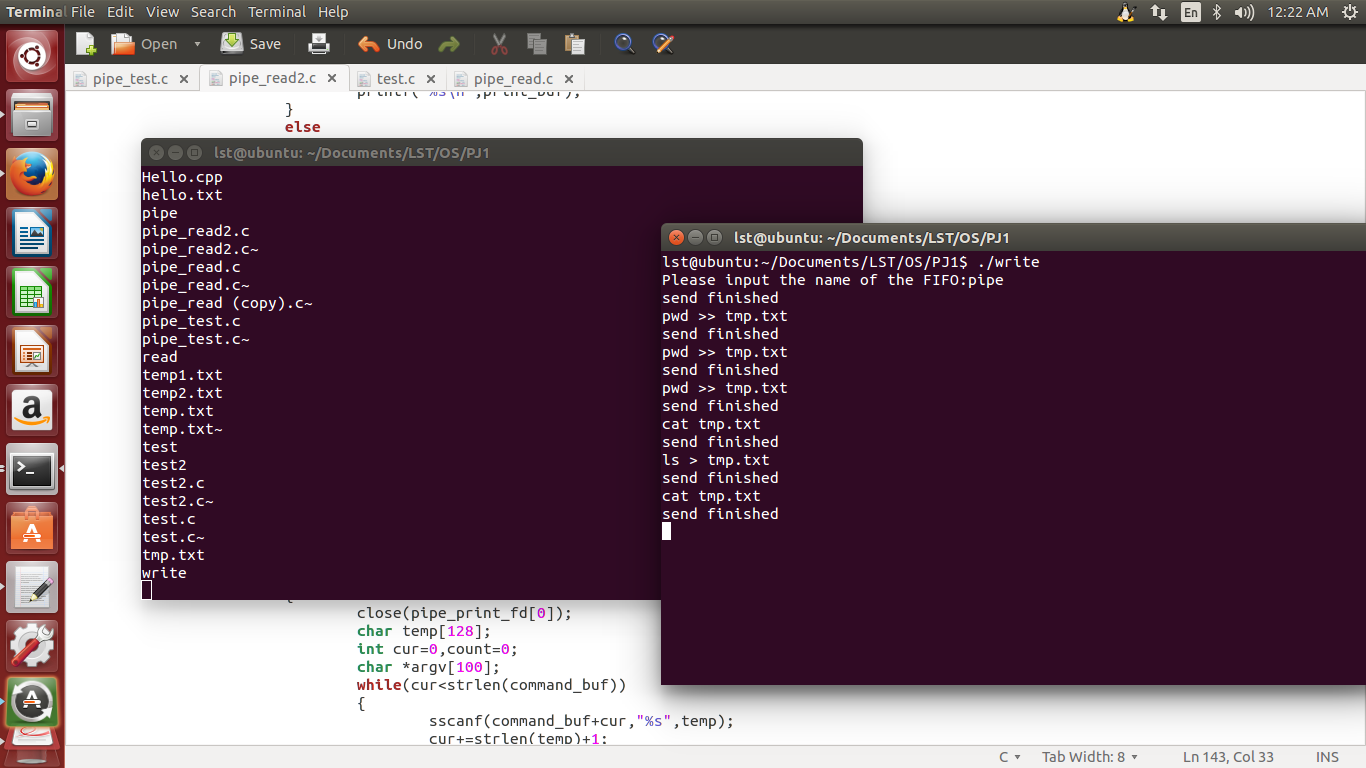
\includegraphics[width =400pt ,keepaspectratio ]{3.png}
\caption{Output Redirection}
\end{figure}
\subsection{Command line pipe}
The commandline pipe is also suported in the program. And the usage is the same as the usual case in Linux. I use several command as examples as shown in Figure\ref{fig:d}.
\begin{figure}[htbp]
\label{fig:d}
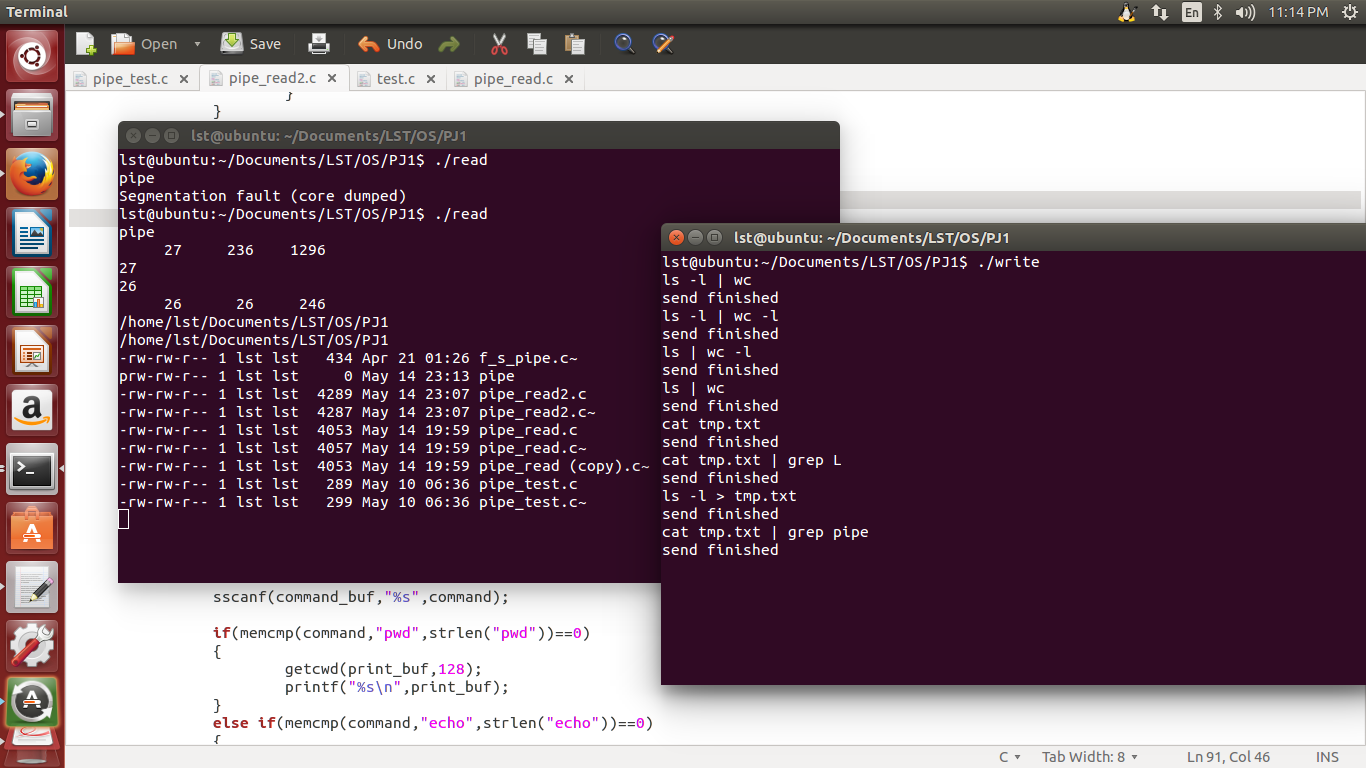
\includegraphics[width =400pt ,keepaspectratio ]{4.png}
\caption{Command Line Pipe}
\end{figure}
\section{Structure of the Program}
The basic and structure of th Program can be shown in the pesudo code of Algorithm\ref{alg:a}
\begin{algorithm}[htbp]  
\label{alg:a}
\caption{Simple Shell Program}
\begin{algorithmic}[1]
\While {true}
\State read from the FIFO to fifobuf
\State search for $'<','>','>>','|'$
\If{there is a redirection}
\State dup2(outputfile,stdout)
\EndIf
\If{there is a command line pipe}
\State devide the command and make the flag
\EndIf
\If{Internal Command}
\State execute the internal command
\Else
\State create a child process
\If {is child process}
\If {there is a command line pipe}
\State create a pipe
\State create a grandchild process
\If {is grandchild process}
\State redirect the stdout to the pipe
\State execute the command before $'|'$
\Else 
\State wait
\State redirect the stdin to the the pipe
\EndIf
\EndIf
\State execute the command 
\Else
\State wait
\EndIf
\EndIf
\State recover the stdin and stdout
\EndWhile
\end{algorithmic}
\end{algorithm}
\section{Conclusion and Future Plan}
\subsection{About the External Commands}
When resolving the externa commands, I used the fork() system call to create a child process, and the child process execute the command. Probably a more right way to use a pipe and redirect the stdout of the child process to the write port of the pipe and let the father process to print the result. However, this method has a fatal problem, there are some commands like ``vim'' that require that the output should be a terminal, not a pipe. So I aborted this method in the final version. However, you can still see it in the annotation in the source codes.
\subsection{About the Redirection of the Input}
The input redirection is also considered in the program but I did not do enough test.
\subsection{Future Plan}
To be determined. 
\end{document}